\section{Разработка эмуляционной игровой среды и методов тестирования}

\subsection{Проектирование и реализация среды игрового процесса}
В выпускной квалификационной работе был поставлен эксперимент по сравнению и оценке качества нейросетевого метода тестирования игрового процесса, в котором для наглядности была разработана эмуляционная игровая среда \textit{Race Against the Machine} "--- аркадная гоночная игра, включающая в себя несколько трехмерных локаций, созданных по образцу существующих районов Санкт-Петербурга и Алматы.

В качестве игрового движка была выбрана мультиплатформенная среда разработки \textit{Unity 2021.3.14f1}, позволяющая создавать трехмерные (3D) и двухмерные (2D) игры, а также интерактивные симуляции и другие неигровые приложения. В качестве вспомогательных библиотек были использованы \textit{DOTween} (объектно-ориентированный анимационный движок с открытым исходным кодом), \textit{ProBuilder} (создание, редактирование и текстурирование пользовательской геометрии внутри \textit{Unity}) и \textit{Cinemachine} (модули для работы с камерой, часто используемые в 3D-анимации).

\begin{figure}
	\centering
	\includegraphics[width=0.75\textwidth]{images/Screenshot\_1920x1080\_29}
	\caption{Кадр геймплея на локации \textit{<<Mountain City Driveway>>}}
	\label{fig:mcdScreenshot}
\end{figure}

\begin{figure}
	\centering
	\includegraphics[width=0.75\textwidth]{images/Screenshot\_1920x1080\_31}
	\caption{Результаты игроков в меню <<Rankings>>}
	\label{fig:rankings}
\end{figure}

Игроком (агентом) в \textit{Race Against the Machine} выступает электромобиль (Рисунок~\ref{fig:mcdScreenshot}). Цель игры -- пройти заданное количество кругов за минимально возможное время. Результаты загружаются на сервер и становятся доступными другим игрокам через меню <<Rankings>> (Рисунок~\ref{fig:rankings}).

Команды агенту (класс \verb|CarController|) могут передаваться как напрямую c помощью выбранного устройства ввода, так и через класс \verb|CarAgent|, выступающий в качестве обертки для нейросети. Архитектура решения представлена на рис.~\ref{fig:diagram}.

\begin{figure}
	\centering
	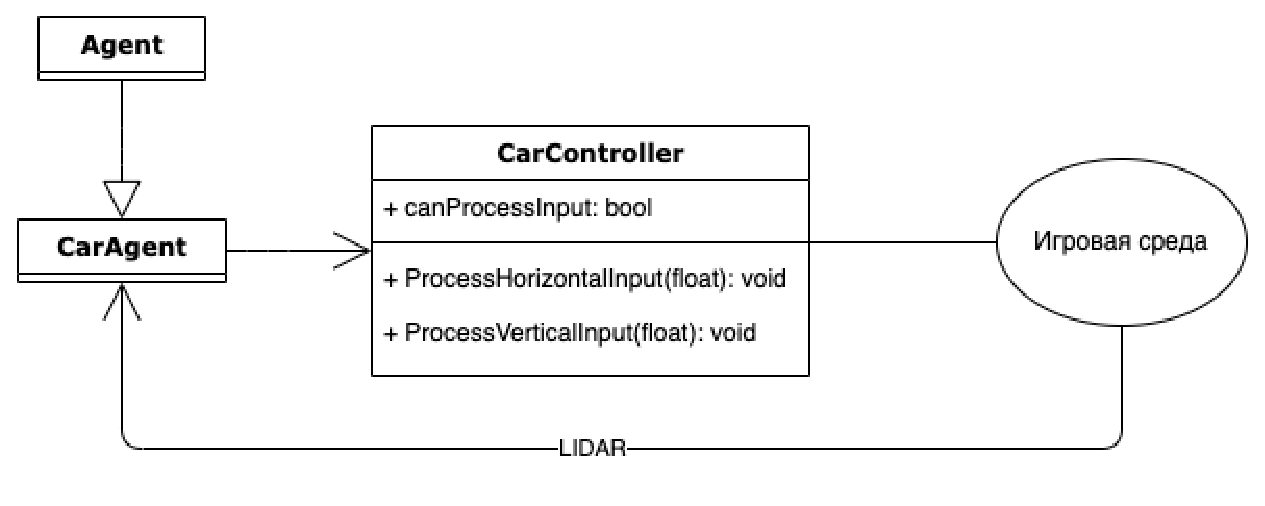
\includegraphics[width=0.75\textwidth]{images/diagram.drawio.eps}
	\caption{Схематическое изображение основной архитектуры проекта}
	\label{fig:diagram}
\end{figure}

Код реализации доступен в открытом репозитории на GitHub \cite{ratm}.

\subsection{Разработка нейросетевего метода тестирования игрового процесса}
В данной работе были рассмотрены подходы к тестированию игрового процесса по компактным представлениям состояний, основанные на следующих нейросетевых архитектурах: \textit{Proximal Policy Optimization} (\textit{PPO}) \cite{ppo} и \textit{Soft Actor-Critic} (\textit{SAC}) \cite{sac}.

В основе \textit{PPO} лежит консервативное обновление политики, ограничивающее соотношение между текущей и прежней политикой в диапазоне \([1-\varepsilon, 1+\varepsilon]\) (\(\varepsilon\) является гиперпараметром). Таким образом мы устраняем стимул, побуждающий нынешнюю политику слишком далеко отходить от предыдущей на каждой эпохе обучения. Функция потерь в архитектуре \textit{PPO} выглядит следующим образом:
\begin{equation}
	L^{\textit{CLIP}}(\theta) = \hat{E}_t[\min(r_t(\theta)\hat{A}_t, \textit{clip}(r_t(\theta), 1 - \varepsilon, 1 + \varepsilon)\hat{A}_t)],
\end{equation} где 
\begin{itemize}
	\item[--] \(\theta\) -- параметр политики;
	\item[--] \(r_t(\theta) = \frac{\pi_\theta(a_t \mid s_t)}{{\pi_\theta}_{old}(a_t \mid s_t)}\) -- отношение вероятностей при новой и старой политиках соответственно. Если \(r_t(\theta) > 1\), то действие \(a_t\) в состоянии среды \(s_t\) более вероятно в текущей политике, чем в предыдущей. В противном случае, если \(r_t(\theta) \in [0, 1]\), то данное действие в текущей политике будет менее вероятным;
	\item[--] \(\hat{E}_t\) обозначает математическое ожидание;
	\item[--] \(\hat{A}_t\) -- оценка <<преимущества>> (\textit{advantage}), которое агент получает при следовании политике \(\pi_\theta\). При \(\hat{A}_t > 0\) действие \(a_t\) в состоянии среды \(s_t\) дает лучший результат по сравнению с другими действиями в этом же состоянии.
\end{itemize}

Беря минимум, мы получаем нижнюю (пессимистическую) границу целевой функции, неограниченной диапазоном \([1-\varepsilon, 1+\varepsilon]\).

% TODO: картиночки!
В рамках эксперимента также была проведен поиск оптимальных значений гиперпараметров \(\varepsilon\) и \(\beta\), используемых в алгоритме. Результат оптимизации путем поиска по решетке приведен на рис.~\ref{fig:hyperopt}.

Этап тренировки агента был организован следующим образом:
\begin{itemize}
	\item[--] в начале каждой эпохи нейросетевой агент инициализировался случайным образом внутри параллелепипеда, ограничивающего игровое поле (Рисунок~\ref{fig:bounds}). Местом возникновения агента обязательно являлось дорожное полотно;
	\item[--] в течение 10 тысяч шагов (продолжительность эпохи подбиралась эмпирическим путем) агент исследовал игровую среду:
	\begin{itemize}
		\item[а)] в случае первичного нахождения локации вида \textit{out of bounds} агенту присуждалась награда в \(+1\) единицу. Этот вид бага зачастую является более критическим, и поэтому за его нахождение мы даем награду выше;
		\item[б)] в случае первичного нахождения локации вида с низким числом кадров в секунду агенту присуждалась награда в \(+0,1\) единицу. Здесь под <<низким числом>> понимается значение меньше 10 кадров/c, т.е. ниже медианного значения в условиях тренировки, округленного до целого числа. 
	\end{itemize}
	\item[--] по прошествии эпохи позиция и угол поворота агента сбрасывались и инициализировались заново, а веса модели обновлялись с использованием собранных наблюдений.
\end{itemize}

\begin{figure}
	\centering
	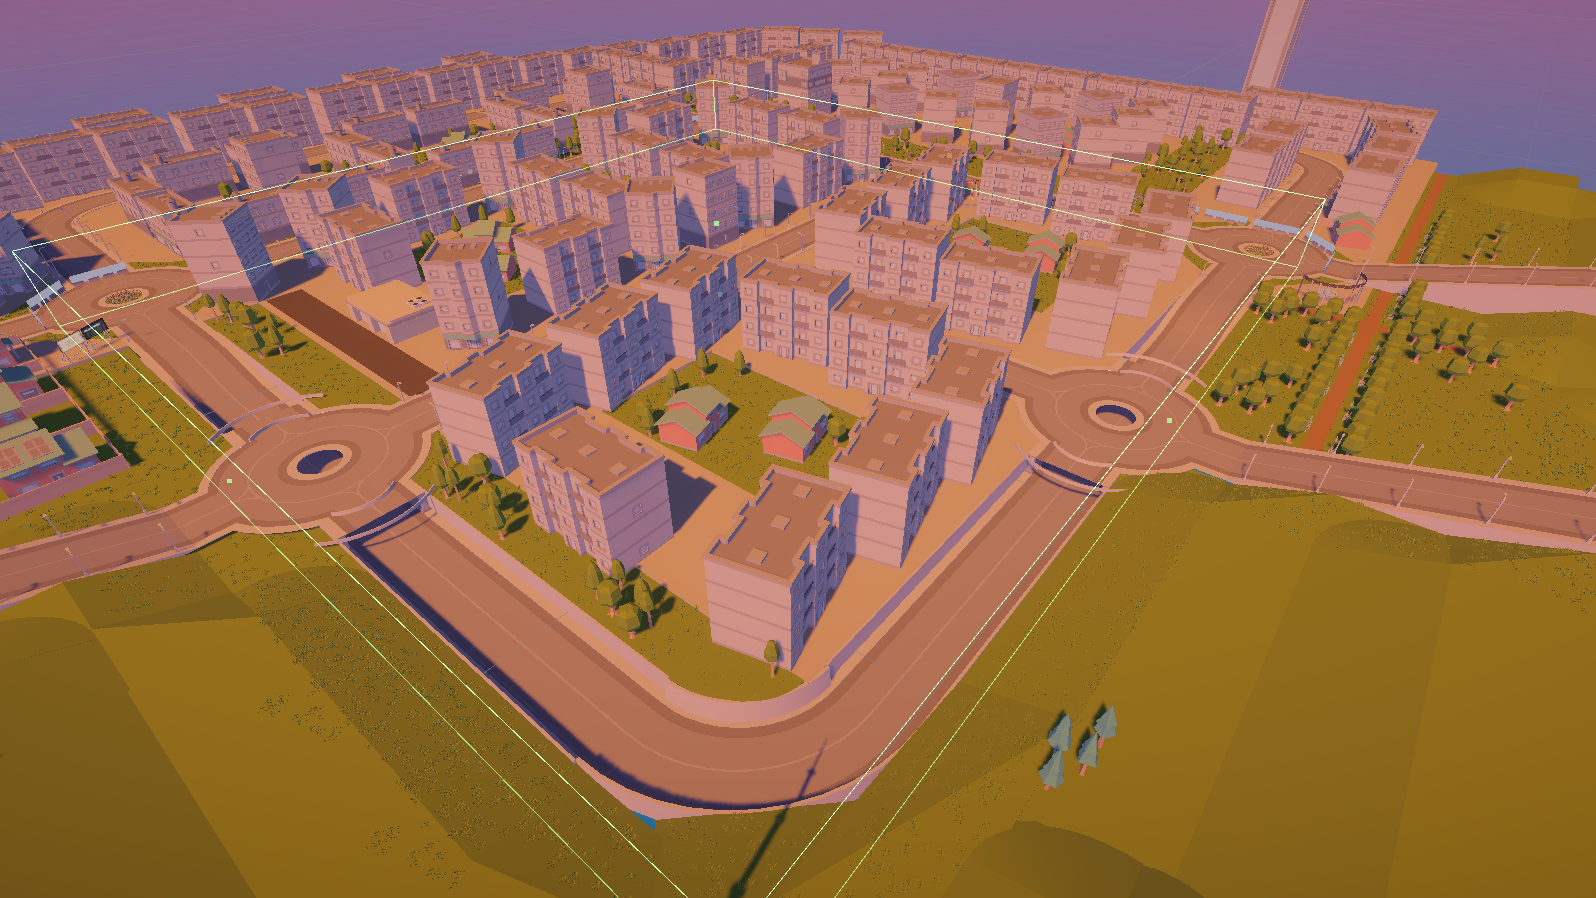
\includegraphics[width=0.75\textwidth]{images/bounds}
	\caption{Границы инициализации игрового агента (отмечены зеленым цветом)}
	\label{fig:bounds}
\end{figure}

\begin{figure}
	\centering
	\includegraphics[width=0.5\textwidth]{images/ppo\_hyperopt}
	\caption{Тепловая карта значений гиперпараметров \(\varepsilon\), \(\beta\) и суммарной награды на момент остановки обучения}
	\label{fig:hyperopt}
\end{figure}

В общем случае нейросетевой агент тренировался 100 эпох (или же, что то же самое, \(10^6\) шагов), и этап тренировки был повторен 10 раз для получения усредненных значений. Графики процесса обучения и функции потерь модели приведены на Рисунках~\ref{fig:training} и~\ref{fig:trainingValueLoss}. 

\begin{figure}
	\centering
	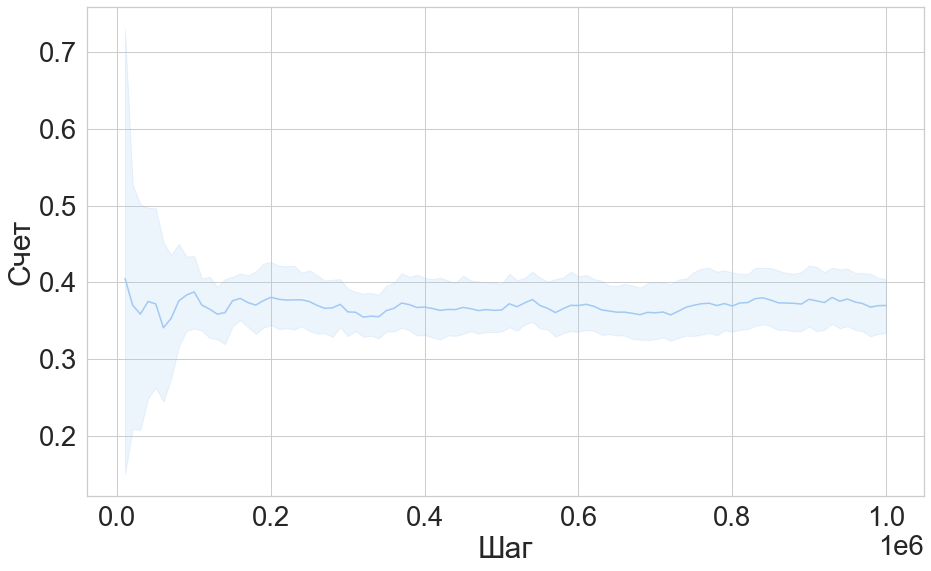
\includegraphics[width=0.75\textwidth]{images/output}
	\caption{Кривая обучения модели в 10 экспериментах. Для каждой эпохи приведены выборочное среднее и 95\%-й доверительный интервал}
	\label{fig:training}
\end{figure}

\begin{figure}
	\centering
	\includegraphics[width=0.75\textwidth]{images/output\_val\_loss}
	\caption{График функции потерь в 10 экспериментах. Для каждой эпохи приведены выборочное среднее и 95\%-й доверительный интервал}
	\label{fig:trainingValueLoss}
\end{figure}

\subsection{Оценка качества и апробация разработанных методов}
Результаты показывают, что получаемое агентом за эпоху среднее значение награды стабилизируется в процессе обучения. Также из Рисунка~\ref{fig:bugLocations} мы видим \(293\) точки на игровой карте, где в ходе одного из тренировочных запусков нейросетевой агент находил оба типа багов. Из карты также видно, что точки формируют <<проблемные>> кластеры: участки с низким числом кадров в секунду концентрируются вокруг травы и деревьев (свидетельство плохой оптимизации игровой зелени), а участки \textit{out of bounds} "--- рядом со зданиями (агент может выйти за пределы игровой среды, прижимаясь к основаниям зданий). Получаемая за найденные ошибки награда отражается в поведении полученного нейросетевого агента: после начала эпохи он стремится на скорости въехать в ближайшие препятствия, пытаясь найти проблемные участки среды.

\begin{figure}
	\centering
	\includegraphics[width=0.75\textwidth]{images/bug\_locations}
	\caption{Лучи исходят из точек на карте, где нейросетевой агент смог найти баги двух видов: \textit{out of bounds} (отмечены голубым) и участки с низким значением \textit{FPS} (отмечены красным)}
	\label{fig:bugLocations}
\end{figure}

%TODO: составить heatmap багов
